% !TEX program = xelatex
%% Requires compilation with XeLaTeX or LuaLaTeX
\documentclass[10pt,xcolor={table,dvipsnames},t]{beamer}
\usepackage[natbib=true,style=authoryear,backend=bibtex,useprefix=true]{biblatex}
\usepackage{caption}
\setbeamertemplate{caption}[numbered]
\addbibresource{reference.bib}
\usepackage{hyperref}
\hypersetup{ 
pdfpagemode=FullScreen,  
colorlinks=true,linkcolor=blue}
\usepackage{enumerate}
\usepackage{algorithm}
\usepackage{algpseudocode}
\usepackage{listings}
\usepackage{xcolor}

\definecolor{codegreen}{rgb}{0,0.6,0}
\definecolor{codegray}{rgb}{0.5,0.5,0.5}
\definecolor{codepurple}{rgb}{0.58,0,0.82}
\definecolor{backcolour}{rgb}{0.95,0.95,0.92}

\lstdefinestyle{mystyle}{
    backgroundcolor=\color{backcolour},   
    commentstyle=\color{codegreen},
    keywordstyle=\color{magenta},
    numberstyle=\tiny\color{codegray},
    stringstyle=\color{codepurple},
    basicstyle=\ttfamily\footnotesize,
    breakatwhitespace=false,         
    breaklines=true,                 
    captionpos=b,                    
    keepspaces=true,                 
    numbers=left,                    
    numbersep=5pt,                  
    showspaces=false,                
    showstringspaces=false,
    showtabs=false,                  
    tabsize=2
}

\lstset{style=mystyle}

% Flow chart config
\usepackage{tikz}
\usetikzlibrary{calc,trees,positioning,arrows,fit,shapes,calc,tikzmark,matrix}
\usepackage{eso-pic}
\usetikzlibrary{shapes.geometric, arrows}
\tikzstyle{startstop} = [rectangle, rounded corners, minimum width=3cm, minimum height=1cm,text centered, draw=black, fill=red!30]
\tikzstyle{io} = [trapezium, trapezium left angle=70, trapezium right angle=110, minimum width=3cm, minimum height=1cm, text centered, draw=black, fill=blue!30]
\tikzstyle{process} = [rectangle, minimum width=3cm, minimum height=1cm, text centered, draw=black, fill=orange!30]
\tikzstyle{decision} = [diamond, minimum width=3cm, minimum height=1cm, text centered, draw=black, fill=green!30]
\tikzstyle{arrow} = [thick,->,>=stealth]

\usetheme{UCBerkeley}

\title[Your Short Title]{STMC HKOI Training}
\subtitle{Lesson 7: String Manipulation (I)}
\author{Chan Yan Mong}
%\institute{}
\date{\today}

\begin{document}

\begin{frame}
  \titlepage
\end{frame}

% Uncomment these lines for an automatically generated outline.
%\begin{frame}{Outline}
%  \tableofcontents
%\end{frame}

\section{Class Goal}

\begin{frame}{Goal today}
String and list are similar so we can do similar operations (Slice, membership, elementwise access etc.) on it. 
\begin{itemize}
  \item Relation between string and list 
  \item ASCII encoding, \texttt{ord()} function
  \item Length, slicing, substring and membership 
  \item Using \texttt{split} and \texttt{join}
  \item Knuth–Morris–Pratt (KMP) algorithm 
\end{itemize}

\end{frame}

\section{Character Encoding}

\begin{frame}[fragile]{Character Encoding}
  \begin{itemize}
    \item In computers, all data are stored as 0s and 1s
    \item Hence, all data stored in computer are fundamentally just numbers 
    \item However, similar to how a string of integers like $21$ can represent either your class number or the money in your pocket, \textit{what a given string of numbers mean are up to us}.
    \item A scheme that assigns numbers to graphical characters is called a \textbf{character encoding}
  \end{itemize}
\end{frame}


\begin{frame}[fragile]{Analogy: Morse Code}
  \begin{columns}
    \begin{column}{0.6\textwidth}
      \begin{itemize}
        \item To illustrate the idea, consider the \textbf{Morse Code}
        \item Can't send characters directly via telegraph
        \item So characters are turned into sequences of two different signal durations, called dots and dashes, that can be sent
        \item To retrieve the characters, people only need to look up what these sequences mean
      \end{itemize}
    \end{column}
    \begin{column}{0.4\textwidth}
      \begin{figure}
        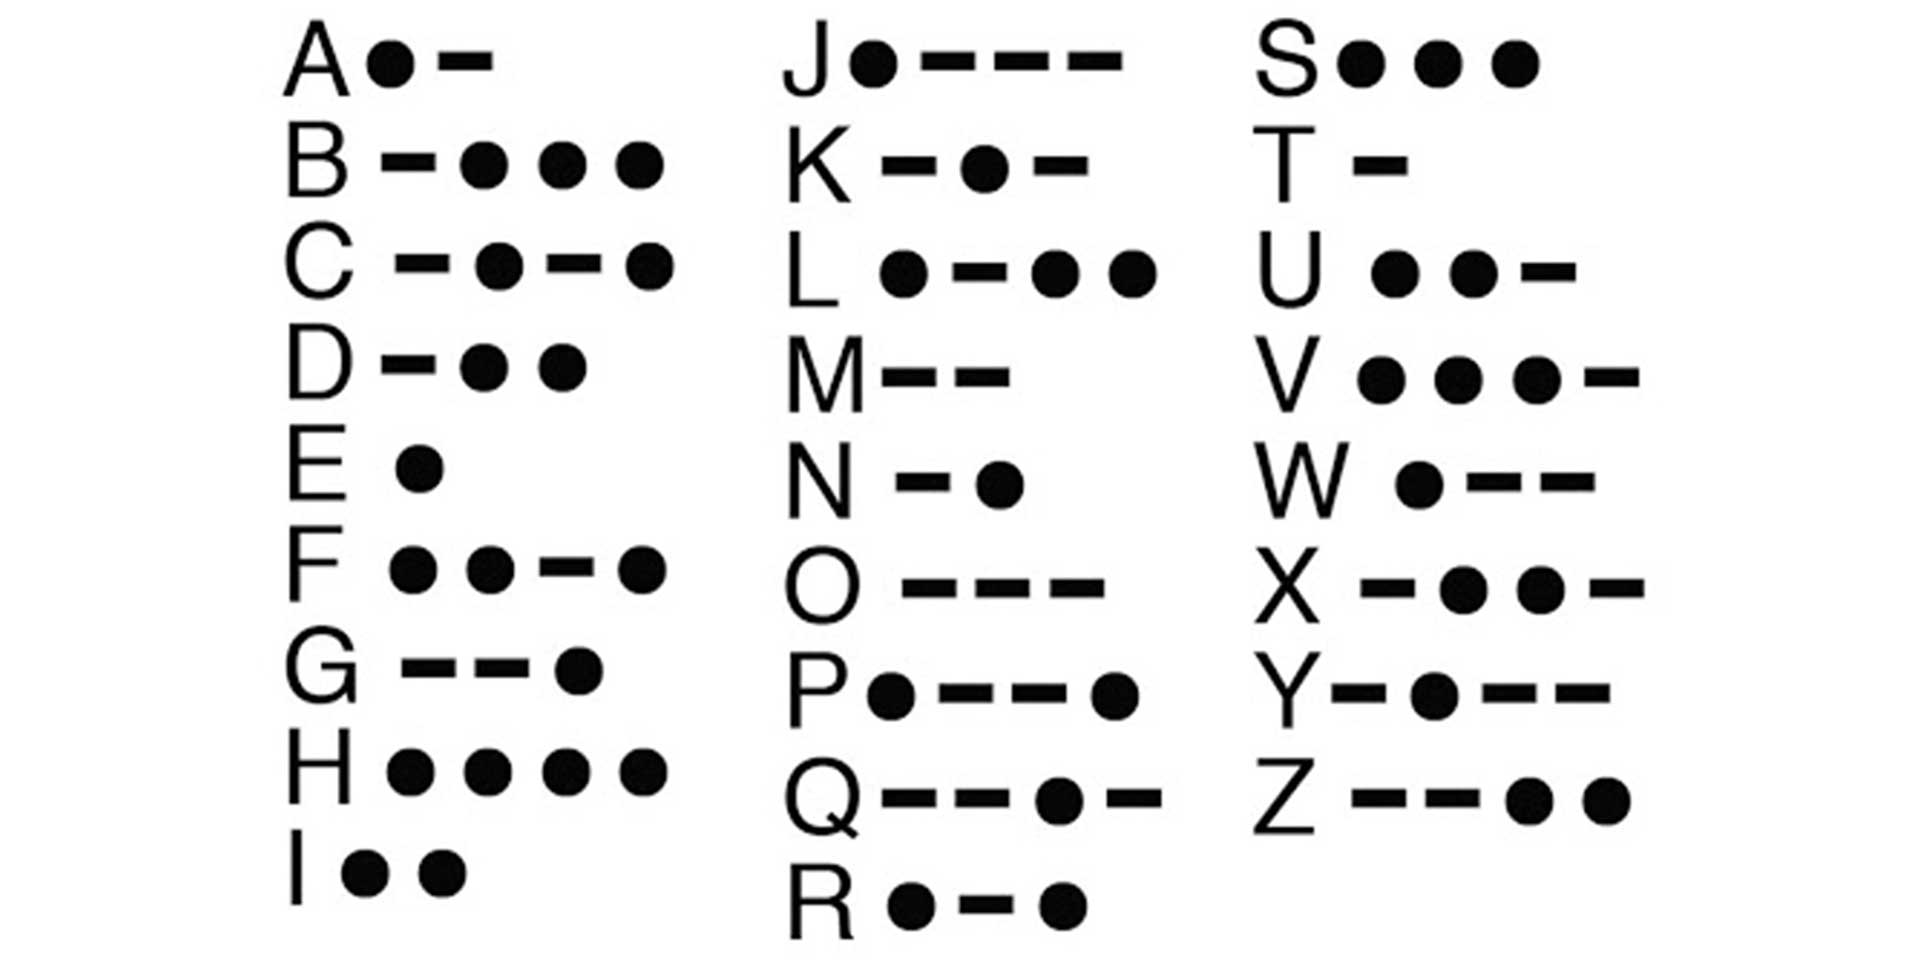
\includegraphics[width=\textwidth]{./img/morse-code.jpg}
        \caption{Morse Code (\href{https://www.discoveryworld.org/about/blog/discover_at_home/morse-code/}{Source})}
      \end{figure}
    \end{column}
  \end{columns}
\end{frame}

\begin{frame}[fragile]{Character Encoding}
  \begin{itemize}
    \item A character encoding does the same thing, except it associate a character with an integer
    \item For example, the ASCII encoding encode \texttt{'A'} with \texttt{65}, \texttt{'B'} with \texttt{66} and etc.
    \item Commonly used character encodings include: \textbf{ASCII}, \textbf{Unicode}, \textbf{Big5}, \textbf{GB}
    \item Here we will focus on \textbf{ASCII}, one of the oldest but also simplest character encoding scheme
  \end{itemize}
\end{frame}

\begin{frame}[fragile]
  Here is the ASCII Table (Source: \href{https://www.alpharithms.com/ascii-table-512119/}{alpahrithms})
  \begin{figure}
    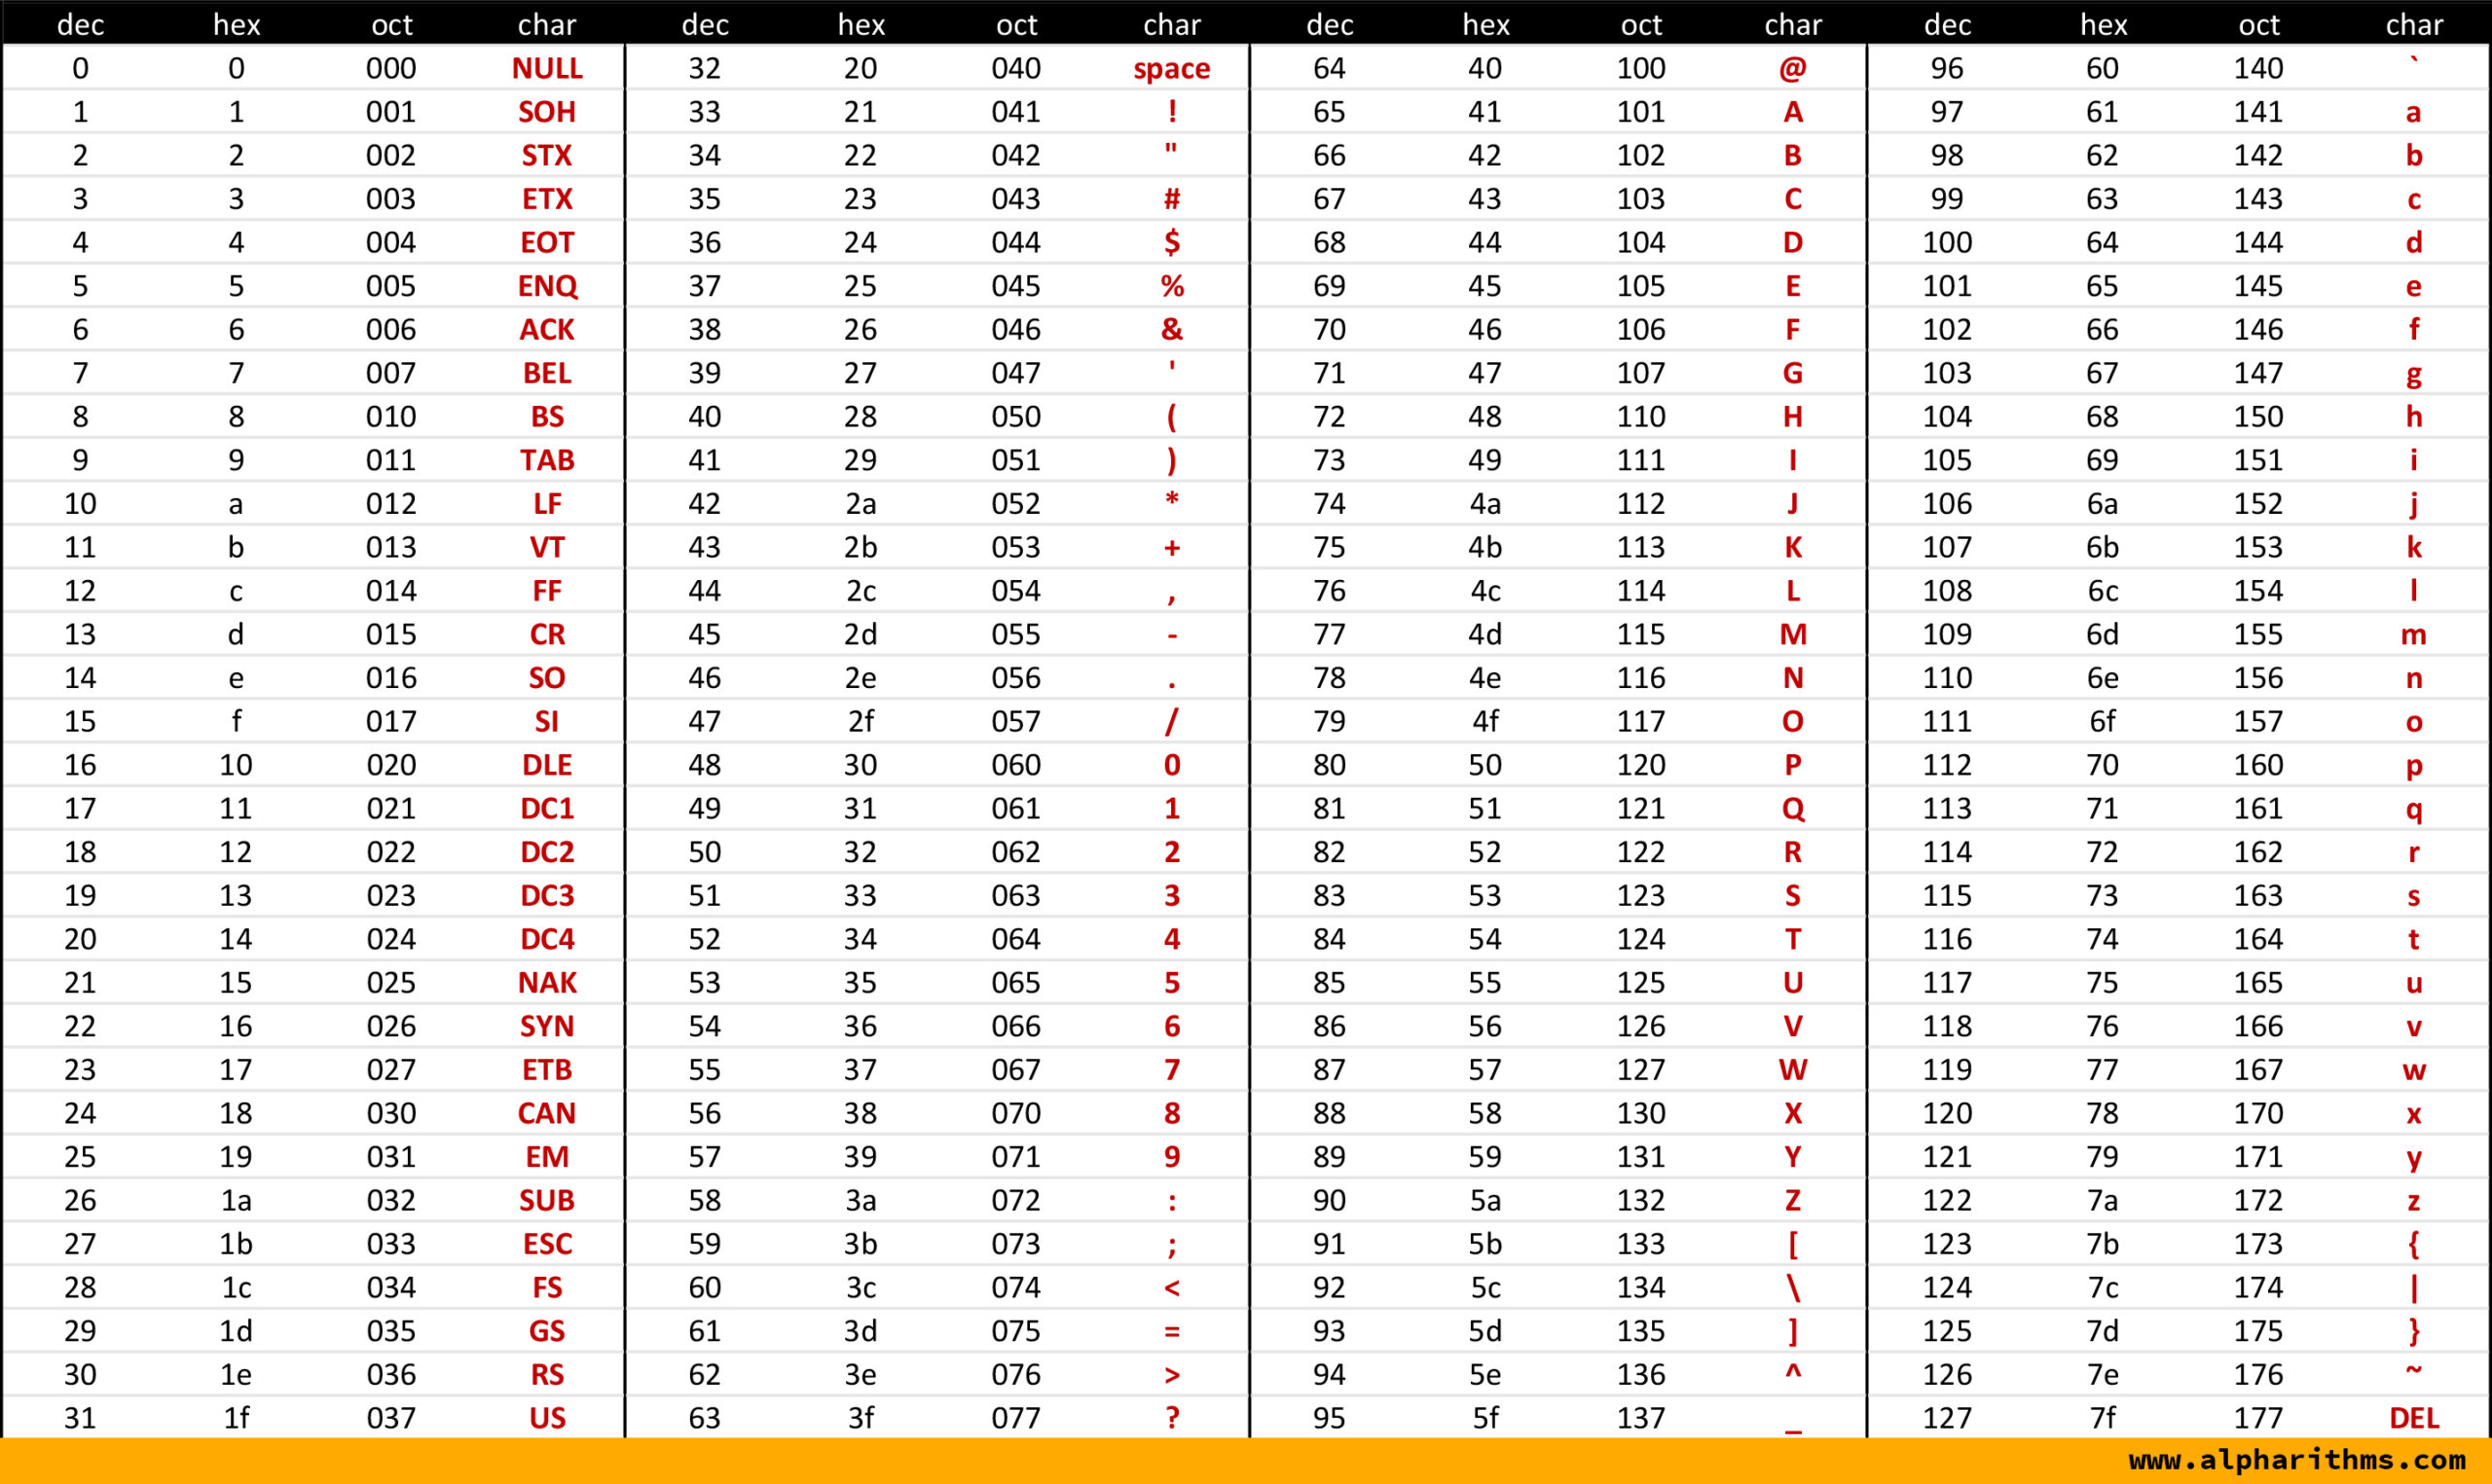
\includegraphics[width=\textwidth]{img/ascii-table.jpg}
  \end{figure}
\end{frame}

\begin{frame}[fragile]{Getting ASCII value using \texttt{ord()}}
  \begin{itemize}
    \item In Python, we can get the ASCII value of a character using \texttt{ord()}
    \item For example: 
\begin{lstlisting}[language=python]
ord('A') # Return 65
ord(' ') # Return 32
ord('a') # Return 97
\end{lstlisting}
    \item \textbf{Exercise:} Using \texttt{ord()}, find the ASCII value of \texttt{'B','c','0','\#','!'}. Compare the results with the ASCII table above
  \end{itemize}
\end{frame}

\section{String and List}
\begin{frame}[fragile]{String and List}
  \begin{itemize}
    \item Now we can understand what actually is a string
    \item Fundamentally, strings are list of characters
    \item Take the string \texttt{"Hello World!"} for example
    \item It can be thought as a list of 12 characters:\\\texttt{['H', 'e', 'l', 'l', 'o', ' ', 'W', 'o', 'r', 'l', 'd','!']}
    \item Therefore, almost all the operations we did with list can be transfered to string
  \end{itemize}
\end{frame}

\begin{frame}[fragile]{Length of String}
  \begin{itemize}
    \item Like list, we can obtain the length of string using \texttt{len()} function
\begin{lstlisting}[language=python]
len('Hello!') # Return 6
len('Python is fun! (Nope)') # Return 21
len('13+19=32') # Return 8
\end{lstlisting}
  \end{itemize}
\end{frame}

\begin{frame}[fragile]{Looping Through String}
  \begin{itemize}
    \item Using this, we can easy loop over strings like we did with list
\begin{lstlisting}[language=python]
myStr = "This is some long long sentence"
for i in range(len(myStr)):
  print(myStr[i]) # Print the string character by character
\end{lstlisting}
    \item For example, we the following code search for the indicies of the character \texttt{'o'}
\begin{lstlisting}[language=python]
myStr = "This is some long long sentence"

for i in range(len(myStr)):
  if myStr[i] == 'o':
    print(f'Find an "o" at: {i}!')
\end{lstlisting}
  \end{itemize}
\end{frame}

\begin{frame}[fragile]{Finding substrings}
  \begin{itemize}
    \item \textbf{Substring} is a continguous sequence of characters within a string 
    \item For example, \texttt{"the best of"} is a substring of \texttt{"it was the best of time"}
    \item In python, we can find the substring using the keyword \texttt{in}. For example:
\begin{lstlisting}[language=python]
"Hire" in "Hire the top freelancers" # True 
"Ben" in "Kelvin is handsome" # False
"Free" in "I am not Free" # True
"may" in "May is a good person" # False
\end{lstlisting}
  \end{itemize}
\end{frame}

\begin{frame}[fragile]{Finding substrings}
  \begin{itemize}
    \item Furthermore, we can get the starting index of the substring using \texttt{find} method
\begin{lstlisting}[language=python]
# Indices  012345678901234567890123456789012345
message = 'Python is a fun programming language'

message.find('fun') # 12
message.find('program') # 16
message.find('language') # 28
\end{lstlisting}
  \end{itemize}
\end{frame}

\begin{frame}[fragile]{Slicing string}
  \begin{itemize}
    \item We can also slice string using similar syntax as that in string 
\begin{lstlisting}[language=python]
  myString[start:end]
\end{lstlisting}
where the \texttt{end} is the index for the end of the slice, with \texttt{end} excluded
    \item For examples:
\begin{lstlisting}[language=python]
# Indices  012345678901234567890123456789012345
message = 'Python is a fun programming language'

message[0:6] # Python 
message[12:15] # fun
message[16:23] # program
\end{lstlisting}
  \end{itemize}
\end{frame}


\begin{frame}[fragile]{Editing characters in strings}
  \begin{itemize}
    \item Strings are \textbf{immutable} in python (unlike in C/C++)
    \item This means the following is invalid:
\begin{lstlisting}[language=python]
myStr = "Hello World"
myStr[0] = 'h' 
# TypeError: 'str' object does not support item assignment
\end{lstlisting}
  \item In general, you cannot modify characters in string directly 
  \item To modify string, one can first convert a string to list and convert it back to string 
  \end{itemize}
\end{frame}

\begin{frame}[fragile]{Editing characters in strings}
  \begin{itemize}
    \item To convert string to list, we can use \texttt{list}
    \item To convert list to string, we can use \texttt{join}
    \item Here is an example:
\begin{lstlisting}[language=python]
myStr = "Hello"
myStr = list(myStr) # ['H','e','l','l','o']
myStr[0] = 'h' # ['h','e','l','l','o']
myStr = ''.join(myStr) # 'hello'
\end{lstlisting}
  \end{itemize}
\end{frame}

\begin{frame}[fragile]{More on \texttt{join} method}
  \begin{itemize}
    \item More generally, the \texttt{join} method takes all items in a list into a string, using \texttt{'sep'} as separator:
\begin{lstlisting}[language=python]
'sep'.join(myList)
\end{lstlisting}
    \item For example: 
\begin{lstlisting}[language=python]
','.join(['May','John','Tim']) # 'May,John,Tim'
' '.join(['May','John','Tim']) # 'May John Tim'
'!!'.join(['May','John','Tim']) # 'May!!John!!Tim'
\end{lstlisting}
  \end{itemize}
\end{frame}


\begin{frame}[fragile]{\texttt{split} method}
  \begin{itemize}
    \item We can also split string into list with separators using the \texttt{split} method
    \item For example: 
\begin{lstlisting}[language=python]
'Tim,Amy,John'.split(',') # ['Tim','Amy','John']
'These are some words'.split(' ') # ['These','are','some','words']
'apple#banana#cherry#orange'.split('#') # ['apple', 'banana', 'cherry', 'orange']
\end{lstlisting}
    \item This is sometimes useful when processing text 
    \item Those who are interested in more advanced text processing should search for \textbf{regex} (regular expression)
  \end{itemize}
\end{frame}

\section{Practicing string handling}

\begin{frame}{Practicing String Handling}
  \begin{exampleblock}{Exercise: King movement}
    HKOI Online Judge (D110): \url{https://judge.hkoi.org/task/D110}
  \end{exampleblock}
  \begin{exampleblock}{Exercise: Phone number}
    HKOI Online Judge (D101): \url{https://judge.hkoi.org/task/D101}
  \end{exampleblock}
  \begin{exampleblock}{Exercise: Bus fare}
    HKOI Online Judge (D102): \url{https://judge.hkoi.org/task/D102}
  \end{exampleblock}
  \begin{exampleblock}{Exercise: String length and words}
    HKOI Online Judge (D302): \url{https://judge.hkoi.org/task/D302}
  \end{exampleblock}
\end{frame}

\section{String Searching}

\begin{frame}{String-Search Algorithms (Optional)}
  \begin{itemize}
    \item The method \texttt{find} is surely a useful string utility provided by python
    \item But \textit{how do they work?}
    \item Here we will introduce a commonly used string search algorithm called \textbf{Knuth–Morris–Pratt (KMP) algorithm}
    \item But first let's try to see how we would approach the problem naively
  \end{itemize}
\end{frame}

\subsection{Naive String Search}
\begin{frame}[fragile]
  \begin{algorithm}[H]
    \caption{Naive String Search}\label{alg:naive_search}
    \begin{flushleft}
      \textbf{Input:} $T[1\cdots n],P[1\cdots m]$ - String and pattern to be searched with length $n$ and $m$ respectively\\
      \textbf{Program:} 
    \end{flushleft}
    \begin{algorithmic}
      \ForAll {$i=1$ to $n-m+1$} 
        \State{$TotalMatch \gets $ True}
        \ForAll {$j=1$ to $m$}
        \If{$T[i+j-1]$ not equal $P[j]$}
          \State{$TotalMatch \gets$ False}
        \EndIf
        \EndFor
        \If{$TotalMatch$ is True}
          \State{Print "A match is found at $s=i$}
        \EndIf
      \EndFor
    \end{algorithmic}
  \end{algorithm}
\end{frame}

\begin{frame}{Naive String Search}
  \begin{itemize}
    \item As one can see, the naive algorithm will run for $(n-m+1)m$ times
    \item So the time complexity is $\mathcal{O}(m(n-m+1))$
    \item As one can see, the algorithm is linear in $n$ but quadratic in $m$, so this is most inefficient when $m \approx n/2$
    \item However, it can be shown that for randomly chosen patterns and text from a set of $d$ alphabets the \textit{expected} number of character-to-character comparison is $\leq 2(n-m+1)$ (See \href{https://www.amazon.com/Introduction-Algorithms-3rd-MIT-Press/dp/0262033844}{Introduction to Algorithms - Problem 32.1-3})
    \item Thus, for randomly chosen strings, the naive algorithm is quite efficient
  \end{itemize}
\end{frame}

\begin{frame}{Why naive algorithm is slow}
  \begin{itemize}
    \item However, we can do better. To see how we can improve, let's first see why the naive algorithm is slow
    \item Our discussion will follow closely that of Ch.32.4 of \textit{Introduction to Algorithms} by Cormen et. al.
    \item The images below are extracted from the book
  \end{itemize}
\end{frame}

\begin{frame}{Why naive algorithm is slow}
  \begin{columns}
    \begin{column}{0.55\textwidth}
      \begin{itemize}
        \item Let $P="\text{ababaca}"$ be the pattern and it aligns with the text $T$ so that
        the first $q=5$ characters match
        \item Now we found that the $6$th character does not match (Connected by zig-zag lines)
        \item We must now shift to the right to find another match
        \item But shift by how much?
      \end{itemize}
    \end{column}
    \begin{column}{0.45\textwidth}
      \begin{figure}
        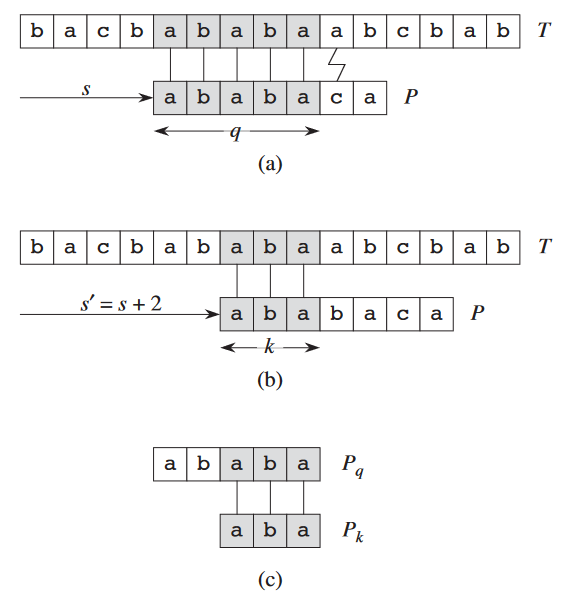
\includegraphics[width=\textwidth]{img/kmp-why-naive-slow.PNG}
      \end{figure}
    \end{column}
  \end{columns}
\end{frame}

\begin{frame}{Why naive algorithm is slow}
  \begin{columns}
    \begin{column}{0.55\textwidth}
      \begin{itemize}
        \item In the \textit{naive} algorithm, we always shift by 1 character ($s' = s+1$)
        \item But as shown in (a), this is inefficient
        \item If we shift $s'=s+1$, the substring in $T$ will be \texttt{"babaabcbab..."}. In other words, it starts with the 2nd character in $P$
        \item But the 2nd character in $P$ is \texttt{"b"} while the first is \texttt{"a"}. There is no way they can match
      \end{itemize}
    \end{column}
    \begin{column}{0.45\textwidth}
      \begin{figure}
        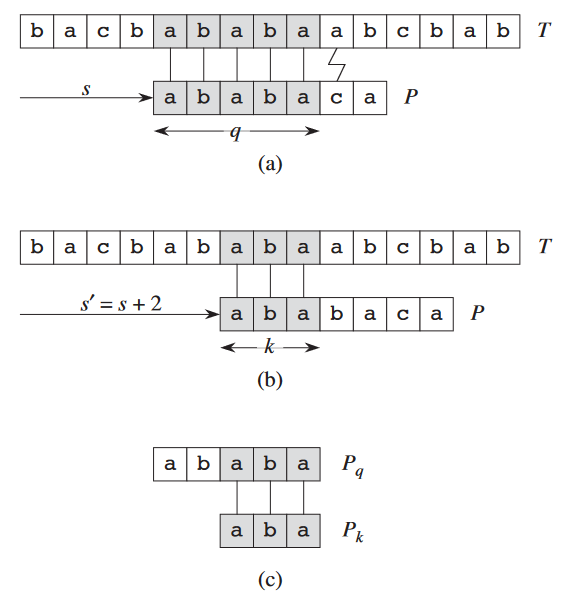
\includegraphics[width=\textwidth]{img/kmp-why-naive-slow.PNG}
      \end{figure}
    \end{column}
  \end{columns}
\end{frame}

\begin{frame}{Why naive algorithm is slow}
  \begin{columns}
    \begin{column}{0.55\textwidth}
      \begin{itemize}
        \item Instead, we can be more efficient by shifting $s'=s+2$ (See (b))
        \item Shifting more allow us to check less before hitting the end of the string. This speeds up the algorithm
        \item Furthermore we also found that the first $k$ has been matched, so we can sart checking from $s'=s+k+2$
        \item This also speeds up the computation
      \end{itemize}
    \end{column}
    \begin{column}{0.45\textwidth}
      \begin{figure}
        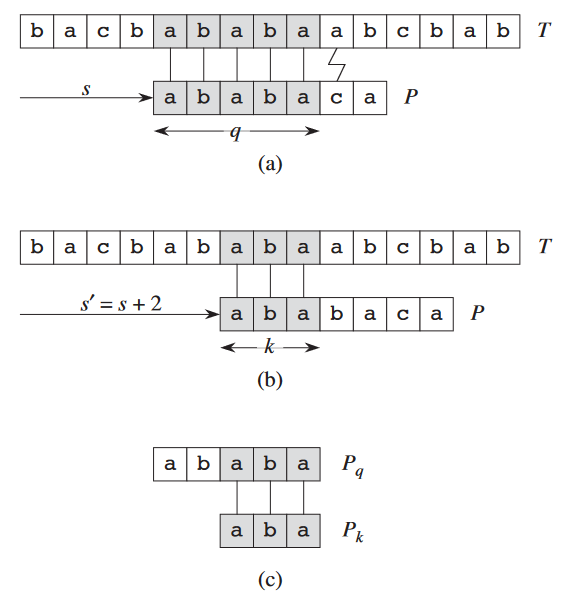
\includegraphics[width=\textwidth]{img/kmp-why-naive-slow.PNG}
      \end{figure}
    \end{column}
  \end{columns}
\end{frame}


\begin{frame}{How many characters to skip?}
  \begin{itemize}
    \item Now comes the question: \textit{How many character should I skip?} 
    \item More importantly: \textit{Can I precompute them using only the pattern string $P$}?
    \item To answer these problems we can consider some examples.
  \end{itemize}
\end{frame}

\begin{frame}{How many characters to skip}
  \begin{exampleblock}{Example: $T=bacbabababacaab$; $P=ababaca$}
    \begin{figure}
      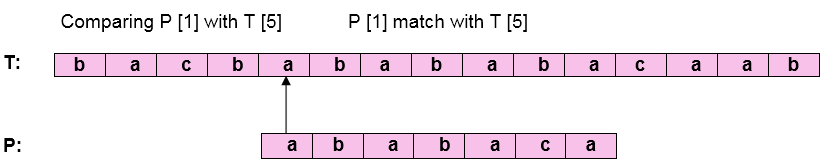
\includegraphics[width=0.8\textwidth]{img/kmp-eg1-01.png}
    \end{figure}
  Extracted from \href{https://www.javatpoint.com/daa-knuth-morris-pratt-algorithm}{javatpoint (KMP algorithm)}
  \end{exampleblock}
\end{frame}

\begin{frame}{How many characters to skip}
  \begin{figure}
    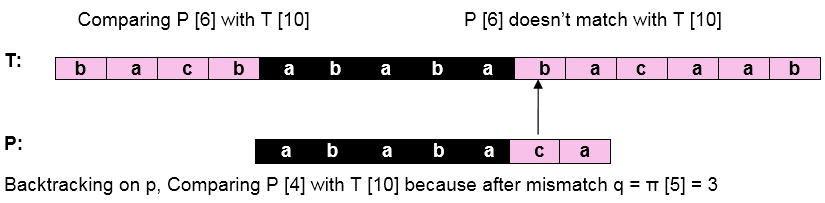
\includegraphics[width=0.8\textwidth]{img/kmp-eg1-02.png}
  \end{figure}
  Extracted from \href{https://www.javatpoint.com/daa-knuth-morris-pratt-algorithm}{javatpoint (KMP algorithm)}
\end{frame}

\begin{frame}{How many characters to skip}
  \begin{itemize}
    \item This example lead us to the following observations
    \begin{itemize}
      \item Given that the pattern characters $P[1\cdots q]$ match text characters $T[s+1\cdots s+q]$, then:
      \item Naively, to skip the most characters, we would like to mentally shift $P[1\cdots q]$ to the end of $T[s+1\cdots s+q]$
      \item But this is wrong, because we might skip useful characters
      \item So we go backward, trying to match the back of $P[1\cdots q]$ with the head of $P[1\cdots q]$ as much as possible
      \item That is, we want to shift by an amount $\pi[q]$ such that:
      \begin{align*}
        \boxed{\pi[q] = \max \{k: k < q \quad \text{and} \quad P[1\cdots k] \text{ is a suffix of } P[1\cdots q]\}}
      \end{align*}
      \item This is the key to \textbf{Knuth–Morris–Pratt algorithm}
    \end{itemize}
  \end{itemize}
\end{frame}

\subsection{Knuth-Morris-Pratt Algorithm}

\begin{frame}[fragile]{Knuth–Morris–Pratt algorithm (Optional)}
  \begin{itemize}
    \item The KMP algorithm was developed by James H. Morris and independently discovered by Donald Knuth. Morris and Vaughan Pratt published a technical report in 1970 ("Knuth–Morris–Pratt algorithm", Wikipedia)
    \item The worse case time complexity is $\Theta(m)+\Theta(n)$
  \end{itemize}
\end{frame}

\begin{frame}[fragile]
  \begin{algorithm}[H]
    \caption{KMP Match}\label{alg:kmp_algorithm}
    \begin{algorithmic}
      \State{$T[1\cdots n],P[1\cdots m]$}
      \State{$\pi,q \gets \text{Compute-Prefix-Function(P)},0$}
      \ForAll {$i=1$ to $n$} 
        \While{$q>0$ and $P[q+1]\neq T[i]$}
          \State{$q \gets \pi[q]$}
        \EndWhile
        \If{$P[q+1]==T[i]$}
        \State{$q\gets q+1$}
        \EndIf
        \If{$q == m$}
        \State{Print "Pattern occurs with shift " $i-m$}
        \State{$q\gets \pi[q]$}
        \EndIf
      \EndFor
    \end{algorithmic}
  \end{algorithm}
\end{frame}

\begin{frame}[fragile]
  \begin{algorithm}[H]
    \caption{Compute Prefix Function}\label{alg:kmp_prefix}
    \begin{algorithmic}
      \State{$P[1\cdots m],\pi[1\cdots m] \gets \text{Empty List}$}
      \State{$\pi[1] = 0$}
      \State{$k=0$}
      \ForAll {$q=2$ to $m$} 
        \While{$k>0$ and $P[k+1]\neq P[q]$}
          \State{$k \gets \pi[k]$}
        \EndWhile
        \If{$P[k+1]==P[q]$}
        \State{$k\gets k+1$}
        \EndIf
        \State{$\pi[q]\gets k$}
      \EndFor
      \State{Return $\pi$}
    \end{algorithmic}
  \end{algorithm}
\end{frame}
\end{document}
